\section{Motivation}\label{sect:seapp_motiv}

As discussed above, \sel and the MAC support have been a crucial
factor in the realization of a secure design and the construction of a
robust app sandbox.  A limitation of the current design is that this
is the only way that apps can benefit from MAC support.  There is
currently no option to let the app developer control the use of the
MAC level, as only platform, vendor, ODM and OEM developers are
allowed to introduce new policy
segments~\cite{seapp_sea_compatibility}.  Our solution overcomes this
limitation, giving the application developer the power to specify new
\sel types and associated permissions.

\subsection{Use cases}\label{sect:seapp_use-cases}
We envision several scenarios that justify the use of \pap.  Many of
them have been previously considered by researchers as motivations for
the introduction in Android of dedicated
components~\cite{seapp_10.1145/2976749.2978333,
  seapp_10.1145/3292006.3300027, seapp_10.1145/3133956.3134064}.

In this section, we give a tour of \pap capabilities using a showcase
app\footnote{The showcase app is available in the \pap repository
  along with the set of modifications to the AOSP.}.  The architecture
of the showcase app is shown in Figure~\ref{fig:seapp_showcase}. Our
description is based on three use cases: fine-granularity in access to
files, fine-granularity in access to services, and isolation of
vulnerability prone components.  Each of the use cases emphasizes the
intra-app security features introduced by \pap.  A dedicated
description, along with policy files that show concretely how to
enforce these use cases, appears in the
Appendix~\ref{appendix:seapp_analysis}; we provide there a technical
demonstration of how \pap can provide protection against a number of
common security problems in Android
apps~\cite{seapp_common_play_protect_vulnerabilites} that were
implemented in the showcase app.

\begin{figure}[h]
	\centering
	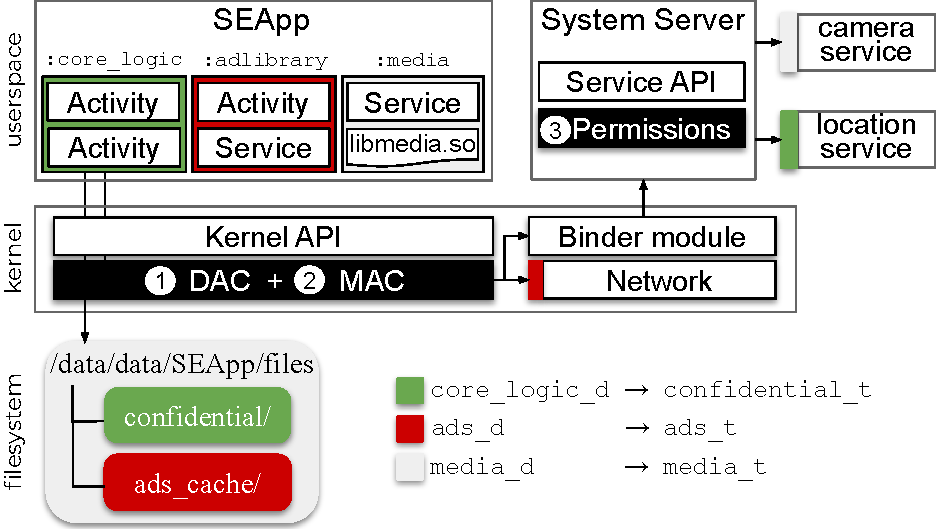
\includegraphics[width=0.8\columnwidth]{chapters/seapp/figs/seapp_showcase_app}
	\caption{\label{fig:seapp_showcase} \bf Security Enhanced App}
\end{figure}

\subsubsection{Fine-granularity in access to files}

Android apps can collect data from multiple sources, and the system
provides many options to store it.  The default one is {\em Internal
  Storage}: a filesystem region, located at \dataappdir, reserved to
each package.  Its content is available to all app's internal
components and inaccessible to any other app.  Since data can be
extremely sensitive, the developer may be interested in restricting
its visibility to only some internal components, labeling sensitive
and non-sensitive data with distinct \sel types (use case 1).  Yet, in
the current Android security model, apps do not have the option to
assign distinct MAC labels to different resources, as all internal
files are labeled \appdatafile.  \pap allows the developer to
introduce dedicated types, and to organize the app's structure with a
separation between components managing non-sensitive data and those
requiring access to sensitive data.  The sensitive components will be
associated with a more stringent MAC domain.
Figure~\ref{fig:seapp_showcase} shows an example in which the {\em
  confidential} files are made accessible to {\em :core\textunderscore
  logic} processes and inaccessible to any other process.

In Appendix~\ref{appendix:seapp_uc1} we give a demonstration of how {\em
  confidential} files are made inaccessible to non-confidential
components in the presence of a path traversal vulnerability.


\subsubsection{Fine-granularity in access to services}

Often developers introduce into their applications code coming from
external sources, which they do not fully trust~\cite{seapp_7958574,
  seapp_10.1145/2414456.2414498, seapp_demetriou2016free}.  For
instance, a common need of app developers is to get revenue from their
apps and a simple approach is to include an Ad delivery library within
the app.  The library is a relatively complex piece of code, with
local computation necessities and the need to manage a dialogue with
remote servers.  The app developer is clearly interested in supporting
the execution of the library, but may want to have guarantees that the
library cannot abuse the access privileges granted by the user to the
whole application sandbox (use case 2).  A common concern is
preventing access to system services such as {\em location}.  These
requirements can be managed by \pap with the definition of a separate
MAC domain for the library.  The process managing the delivery of Ads
will be associated with this domain, which will provide only the
necessary privileges to access the dedicated resources needed for the
library execution.  \sel will then guarantee the confinement of the
library, preventing access to the location service even if the
\texttt{ACCESS\textunderscore FINE\textunderscore LOCATION} permission
is granted to the app.  Figure~\ref{fig:seapp_showcase} shows an
example in which the {\em :adlibrary} process is granted access to the
network but is prevented from accessing \texttt{location service}.

In Appendix~\ref{appendix:seapp_uc2} we give a demonstration of how
the showcase app can support the execution of the Unity
Ads~\cite{seapp_unityads} framework with a dedicated \sel domain. We
also describe in detail how \pap prevents a malicious component, which
was deliberately injected by us into the library process, to capture
the device location.


\subsubsection{Isolation of vulnerability prone
  components}\label{sect:seapp_int_comp_isolation}

App developers often have to consider that the input provided to the
app can come from untrusted sources.  A typical example is the
rendering of complex Javascript code performed by WebView.  The
solution currently offered by Android is to execute these potentially
dangerous actions within a sandbox using {\em isolatedprocess}, i.e.,
a special process that is isolated from the rest of the system and has
no permissions of its own~\cite{seapp_isolatedprocess_perm}.  It runs
under a dedicated UID and \sel domain, and it can only interact with a
restricted number of services~\cite{seapp_isolated_app_te}.

A common need of app developers is to take advantage of complex media
or processing libraries, components that are not considered malicious,
but due to their size and complexity are more likely to have security
bugs.  The developer is then interested in isolating these potentially
vulnerable components (use case 3).  {\em Isolatedprocess} offers a
high protection level in Android, however, its use imposes several
restrictions on the developers.  For instance, {\em isolatedprocess}
cannot perform many of the core Android IPC functions, and the only
way to interact with it is through the bound service
API~\cite{seapp_bound_service_api}.  Also, {\em isolatedprocess} can
only access already open app files received over Binder.  Another
shortcoming is that each invocation of an {\em isolatedprocess}
requires the creation of a new process.  If a series of requests are
made by the app, the performance impact can be significant.  \pap
offers an easier way to do this compared to {\em isolatedprocess}, as
it permits to assign a domain to the process in which the component is
executed, and then configure the required permissions at MAC level.
In terms of performance, the management of multiple requests does not
require the system to activate a new process with a new UID and a
dedicated \sel category.  Figure~\ref{fig:seapp_showcase} shows how to
confine the {\em :media} component.

In Appendix~\ref{appendix:seapp_uc3} we give a demonstration of how
the showcase app can support the execution of media components relying
on a native library in a dedicated process. We also describe how the
developer can leverage \pap to prevent the code of the library from
the execution of unwanted or unintended operations, like opening a
network connection.


\subsection{Modular app compartmentalization}

The motivations presented above become more frequent as apps increase
their size and complexity, and several important apps see a continuous
increase in these parameters.  For instance, Facebook Messenger
version 285 contains more than 500 components and WhatsApp Messenger
version 2.20 more than 300.  This increase in size and the need to
manage it is testified by the development of App
Bundles~\cite{seapp_app_bundles}, Android's new, official publishing
format that offers a more efficient way to build and release modular
applications.

In these large and modular apps, developers find it difficult to fully
control which components of an app are using sensitive
data\footnote{The topic was explicitly considered
  in~\cite{seapp_burke_interview}, an interview with Android's VP of
  Engineering.}.  The availability of a solution such as \pap can
greatly reduce such risk.  A better compartmentalization can reduce
the impact of internal vulnerabilities in modular apps, since each
module can be associated with a dedicated policy fragment.  From a
security and software engineering standpoint, \pap permits to separate
the activities of security policy maintenance and development of new
features.

\subsection{Compatibility with Android design}

Looking at the evolution of Android, it is clear that our proposal is
consistent with the evolution of the operating system and the desire
of its designers to let app developers have access to an extensive and
flexible collection of security tools.  The major obstacles, as
perceived by OS developers, on offering to app developers the use of
MAC services are: weakening of the protection of system components;
performance impact; usability by app developers.  The work we did
solves these concerns: our approach guarantees that app policies do
not have an impact on the system policy
(Section~\ref{subsect:seapp_constraints}); the app policy can be
specified declaratively and attention has been paid to let developers
adopt the approach in a convenient way
(Section~\ref{subsect:seapp_structure}); and, experiments demonstrate
the acceptable performance impact, with a quite limited overhead at
app installation time, and a negligible runtime impact
(Section~\ref{sect:seapp_performance}).

\subsection{Compatibility with other proposals}
As presented in Section~\ref{sect:seapp_use-cases}, \pap by itself
provides protection against a broad spectrum of attacks (see
Appendix~\ref{appendix:seapp_analysis}), but its merit does not end
there.  As multiple literature proposals (e.g.,
\cite{seapp_10.1145/3133956.3134064, seapp_boxify, seapp_aframe})
build upon process isolation and use it to accomplish separation of
privileges at the application layer, \pap could be used as building
block to enforce such restrictions at the MAC layer too, enabling
defense in depth. Moreover, SEApp could also work in conjunction with
other solutions that work at MAC level such as {\em
  FlaskDroid}~\cite{seapp_flaskdroid}, to benefit of its Userspace
Object Managers (USOMs) coverage of the Android system services and
provide finer granularity in access to services.


%%% Local Variables: 
%%% mode: latex
%%% TeX-master: "../../../main.tex"
%%% reftex-default-bibliography: "../../../bib/biblio.bib"
%%% End:
